\documentclass{ufsctex/ufsctex}

\usepackage{graphicx, enumitem, listings, float, pgfplots}
\graphicspath{{./images/}}
% Copyright 2017 Sergei Tikhomirov, MIT License
% https://github.com/s-tikhomirov/solidity-latex-highlighting/

\usepackage{listings, xcolor}

\definecolor{verylightgray}{rgb}{.97,.97,.97}

\lstdefinelanguage{Solidity}{
	keywords=[1]{anonymous, assembly, assert, balance, break, call, callcode, case, catch, class, constant, continue, constructor, contract, debugger, default, delegatecall, delete, do, else, emit, event, experimental, export, external, false, finally, for, function, gas, if, implements, import, in, indexed, instanceof, interface, internal, is, length, library, log0, log1, log2, log3, log4, memory, modifier, new, payable, pragma, private, protected, public, pure, push, require, return, returns, revert, selfdestruct, send, solidity, storage, struct, suicide, super, switch, then, this, throw, transfer, true, try, typeof, using, value, view, while, with, addmod, ecrecover, keccak256, mulmod, ripemd160, sha256, sha3}, % generic keywords including crypto operations
	keywordstyle=[1]\color{blue}\bfseries,
	keywords=[2]{address, bool, byte, bytes, bytes1, bytes2, bytes3, bytes4, bytes5, bytes6, bytes7, bytes8, bytes9, bytes10, bytes11, bytes12, bytes13, bytes14, bytes15, bytes16, bytes17, bytes18, bytes19, bytes20, bytes21, bytes22, bytes23, bytes24, bytes25, bytes26, bytes27, bytes28, bytes29, bytes30, bytes31, bytes32, enum, int, int8, int16, int24, int32, int40, int48, int56, int64, int72, int80, int88, int96, int104, int112, int120, int128, int136, int144, int152, int160, int168, int176, int184, int192, int200, int208, int216, int224, int232, int240, int248, int256, mapping, string, uint, uint8, uint16, uint24, uint32, uint40, uint48, uint56, uint64, uint72, uint80, uint88, uint96, uint104, uint112, uint120, uint128, uint136, uint144, uint152, uint160, uint168, uint176, uint184, uint192, uint200, uint208, uint216, uint224, uint232, uint240, uint248, uint256, var, void, ether, finney, szabo, wei, days, hours, minutes, seconds, weeks, years},	% types; money and time units
	keywordstyle=[2]\color{teal}\bfseries,
	keywords=[3]{block, blockhash, coinbase, difficulty, gaslimit, number, timestamp, msg, data, gas, sender, sig, value, now, tx, gasprice, origin},	% environment variables
	keywordstyle=[3]\color{violet}\bfseries,
	identifierstyle=\color{black},
	sensitive=false,
	comment=[l]{//},
	morecomment=[s]{/*}{*/},
	commentstyle=\color{gray}\ttfamily,
	stringstyle=\color{red}\ttfamily,
	morestring=[b]',
	morestring=[b]"
}

\lstset{
	language=Solidity,
	backgroundcolor=\color{verylightgray},
	extendedchars=true,
	basicstyle=\footnotesize\ttfamily,
	showstringspaces=false,
	showspaces=false,
	numbers=left,
	numberstyle=\footnotesize,
	numbersep=9pt,
	tabsize=2,
	breaklines=true,
	showtabs=false,
	captionpos=b
}



\instituicao[a]{Universidade Federal de Santa Catarina}
\departamento[o]{Departamento de Informática e Estatística}
\curso[o]{Programa de Graduação em Ciência da Computação}
\documento[o]{{Trabalho de Conclusão de Curso}}
\titulo{Verificação de eleição utilizando blockchain}
\autor{Vinicius Macelai}
\grau{Bacharel em Ciência da Computação}
\local{Florianópolis}
\data{01}{novembro}{2019}
\orientador[Orientador]{Prof.\ Dr.\ Jean Everson Martina}
\coordenador[Coordenador]{Prof.\ Me.\ José Francisco Danilo de Guadalupe Correa
Fletes}

\numerodemembrosnabanca{2}
\orientadornabanca{nao}
\coorientadornabanca{nao}
\bancaMembroA{Me. Fernando Pereira \\
  Universidade Federal de Santa Catarina
}
\bancaMembroB{Gustavo Zambonim \\
  Universidade Federal de Santa Catarina
}

\dedicatoria{A todas as pessoas que eu amo}

\agradecimento{Agradeço à minha família, que desde sempre me incentivou e me
deu todo o suporte necessário nessa longa caminhada de estudos. Sem esse apoio,
nada disso seria possível. Em especial a Bruna Luiza, que sempre tentou me
manter motivado e dando apoio em todas formas possíveis.

Agradeço ao meu orientador Jean Martina, por todo o conhecimento compartilhado
e incentivar a busca por aprimoramente pessoal.

Ao LabSEC por ter me acolhido e contribuir para a minha formação acadêmica e
profiossional, além de, toda a amizade que construi com os colegas em as
diversas idas ao Restaurante Universitário.

Aos amigos que fiz durante a graduação, que fizeram parte dessa jornada,
passando muito tempo jogando no Centro Acadêmico, ao companheirismo durante as
matérias e tantas outras coisas que se passa durante uma graduação.

E não menos imporatnte aos amigos do futebol de quinta, que forneceram uma
válvula de escape para momentos cômicos e de vital importância a toda essa
caminhada.
}

\epigrafe{\emph{“We shall meet in the place where there is no darkness.”} \\
	- \textit{George Orwell, 1984}
}

\textoResumo{As abordagens utilizadas  nos sistemas de eleição da maioria dos
países continuam a ser realizadas de  forma manual, com cédulas na forma de
papel. Tal modelo traz problemas enormes de logística e um alto custo para
funcionamento devido aos requisitos de uma eleição segura, que deve fornecer
privacidade, transparência, verificabilidade e confiabilidade. Já as  abordagens
eletrônicas  via internet, ainda carregam desconfiança	sobre manter estas
propriedades.  Uma possível solução para melhorar uma abordagem eletrônica seria
utilizar uma blockchain para melhorar sua auditabilidade, que é o ponto mais
questionado nesse esquema. A blockchain possui propriedades intrínsecas, como a
imutabilidade dos dados, e com esquemas utilizando contratos inteligentes na
blockchain é possível realizar a verificação dos votos de forma descentralizada
e  aberta ao público. Assim, cria-se um sistema que mantém as propiedades
citadas anteriormente, com um baixo custo e menor necessidade de confiar em uma
entidade central.} 
\palavrasChave{criptografia, eleições, democracia,
blockchain, contratos inteligentes}

\textAbstract{As approaches used in the selection systems of most remaining
countries an executed service manual with paper banknotes. Such a model brings
huge logistical problems and a high cost of operation due to requirements of a
safe selection, which should provide privacy, transparency, verifiability and
requirements. Already the electronic approaches via internet, still carry
distrust about maintaining these properties.  A possible solution to improve an
electronic approach would be to use a blockchain to improve your auditability,
which is the most questioned point in this scheme. A blockchain has intrinsic
properties such as data immutability and schemas smart contracts on blockchain
it is possible to check votes decentralized and open to the public. Thus, a
system is created that maintains as properties mentioned above, with a low cost
and the least need to rely on a central entity.}
\keywords{crypto, elections, democracy, blockchain, smart contracts}

\begin{document}

\capa{}

\pretextuais{}

\listadefiguras{}

\listadetabelas{}

\listadeabreviaturas{}

\listadesimbolos{}

\sumario{}

\chapter{Introdução} Ainda que vivamos no momento onde tudo é digital e façamos
as mais diversas tarefas de maneira eletrônica e online, quando o assunto é
votação no meio eletrônico, existem as mais diversas e controversas opiniões a
respeito.

No Brasil, eleições eletrônicas têm sido utilizadas por mais de 20 anos e testes
recentes mostram que, mesmo com o desenvolvimento durante todo esse período, o
atual sistema não consegue se mostrar realmente seguro\cite{aranha}. O maior
problema com a solução proposta pelo Governo Brasileiro é a falta de
auditabilidade, em que só é possível se voluntariar para testar o sistema em um
ambiente controlado. Ainda durante o processo eleitoral, é necessário confiar
cegamente no sistema, não há instrumento nenhum que permita verificar se o voto
foi realmente computado.

Os sistemas de votação eletrônicos atuais se baseiam em esquemas que utilizam de
criptografia homomórfica, que permite que dados cifrados possam ser processados
sem serem decifrados, assim garantindo propriedades importantes para o
sistema.\cite{springer}. Entretanto, esses esquemas são utilizados de forma
centralizada, rodando apenas em um servidor central, sem a possibilidade de tais
informações serem acessadas pelo o público em geral de maneira transparente.

Para realizar a auditoria das votações, é possível utilizar da tecnologia
blockchain, que são bases de registro de dados distribuídos e compartilhados,
desta forma criando um consenso e confiança sobre o estado atual do
sistema.\cite{nakamoto2012bitcoin}.  Garantir essas propriedades intrínsecas,
como a imutabilidade dos dados, é um bom sistema para manter o registro dos
votos, além da possibilidade de rodar contratos inteligentes que podem processar
os votos de maneira descentralizadas junto com a criptografia homomórfica para
garantir o anonimato.

Neste trabalho, optou-se por enfatizar o estudo e a utilização da blockchain e
protocolo Ethereum, a qual fornece contratos inteligentes de alto
nível\cite{ethereum}.  Apresenta-se um esquema que utiliza esses contratos para
garantir as propriedades já citadas, além do estudo de seu impacto financeiro.

Ainda, visa implementar uma solução que integre todas estas partes, um módulo
para um sistema de eleição eletrônico que permite ter informações sobre o
votante de forma confiável. Além disso, almeja possibilitar a realização da
verificação de integridade da eleição, além de detectar alguma tentativa de
mudança dos parâmetros da votação já pré-definidos em uma blockchain de forma
descentralizada e pública.

Por fim, realizar um estudo do custo operacional para rodar tal esquema. De
maneira a definir individualmente cada custo com o esquema proposto e realizar
uma discussão para saber até que ponto seria economicamente viável tal modelo.

\section{Motivação}

Os modelos de eleição utilizados nos dias de hoje são em sua maioria em cédulas
de papel. Dependendo da dimensão da votação, isso externaliza grandes problemas,
no que concerne à logística, que tem como consequência um aumento de custos. Já
as abordagens que utilizam do meio eletrônico e online, geram grande
desconfiança para a maioria das partes interessadas, com receio que o resultado
seja hackeado e alterado. Consequentemente há uma demanda por um modelo de
votação que seja mais auditável e aberto para sanar esse problema de
desconfiança.

\section{Justificativa}

Este tema foi escolhido devido sua grande importância, uma uma vez impacta
basicamente todos os setores da sociedade, pois existem votações nas mais
diversas esferas, desde a governança de empresas, até consultas de opinião sobre
assuntos delicados.  Além dos pontos anteriores citados, a utilização da recente
tecnologia blockchain para a solução destes problemas é uma grande inovação na
área. Este trabalho visa contribuir com modelos mais eficientes e transparentes,
que beneficiarão a sociedade como um todo.

\section{Pergunta de pesquisa}

Este trabalho visa responder se é possível construir um modelo de eleição
eletrônica utilizando a blockchain para garantir uma maior auditabilidade do
sistema. Além de responder até qual volume de dados seria possível processar em
contratos inteligentes na blockchain, juntamente com o cálculo econômico.

\section{Hipóteses}

\begin{itemize}
	\item É possível criar um modelo de eleição eletrônica utilizando blockchain
		para fornecer maior auditabilidade.
	\item É viável utilizar a blockchain Ethereum até qual volume dados.
	\item É economicamente viável esse modelo.
\end{itemize}

\section{Objetivo geral}

Estudar e criar a implementação de um sistema online de eleição, com foco
principal na parte de realizar auditoria e verificação dos votos em blockchain
com auxílio de contratos inteligentes, utilizando um sistema já desenvolvido.
Além disso, analisar as implicações que esse sistema teria no funcionamento e
custos de uma eleição. \\

\section{Objetivo específico}

\begin{enumerate}[label=\roman*.]
	\item Analisar o estado da arte: estudar as principais soluções
	já propostas na literatura com o objetivo de identificar problemas
	e oportunidades para melhorar o trabalho.
	\item Implementar possibilidade de verificação na blockchain:
	Criação de  um módulo para tornar o sistema mais auditável e 
	verificável para o público em geral.
	\item Comparar e analisar as consequências do esquema.
\end{enumerate}

\section{Metodologia}

O trabalho será desenvolvido utilizando a infraestrutura e recursos do
Laboratório de Segurança em Computação (LabSEC/UFSC), em que será estudada a
bibliografia referente aos assuntos abordados nesta pesquisa, visando encontrar
uma abordagem para um sistema de eleição eletrônica com blockchain e contratos
inteligentes.  Frisando suas vantagens e desvantagens e seus custos.

\section{Resultados esperados}

Espera-se contribuir para o estado da arte em eleição eletrônica utilizando
blockchain de forma que aumente a transparência e a auditabilidade do processo.
É esperado também que tal abordagem tenha um gargalo no volume de dados
processados, visto que a tecnologia blockchain por ser descentralizada, não
conseguirá processar diversas transações por segundo. Além de que, como há muito
processamento de dados, devido a criptografia homomórfica, tende a ser inviável
economicamente para casos onde não há necessidade de tanta segurança.

\chapter{Revisão Sistemática}

\section{Descrição}

Este capítulo tem como objetivo realizar uma revisão sistemática do estado da
arte sobre a tecnologia \textit{blockchain} com sua utilização em eleições
eletrônicas, irá ser verificado se já há algum trabalho que tenha o mesmo
objetivo deste, garantir um processo melhor de auditoria utilizando de prova de
existência com a \textit{blockchain}. Foi decidido realizar uma revisão
sistemática para garantir que não haja vieses na revisão do estado da arte. A
revisão sistemática segue um método de seleção e análise de dados e trabalhos
definidos anteriormente da revisão em si, em um processo rígido e bem definido,
evitando vieses.

\section{Definição da estratégia de busca}

A busca foi realizada nos maiores banco de dados de trabalhos científicos
disponíveis, Google Scholar e Scopus. As palavras chaves utilizadas são
\textit{Smart contracts} e \textit{Elections}, dando exclusividade a trabalhos
em inglês. A busca foi reduzida para trabalhos publicados apenas nos anos de
2018 e 2019, para se obter resultados apenas do estado atual. Desta busca,
foram revisados os 10 primeiros trabalhos de cada banco de buscas, da forma que
cada banco de pesquisas tem seu modelo de relevância para determinar as
primeiras colocações, como número de citações e melhor encaixe com as palavras
chaves pesquisadas.

\section{Resultados}

De acordo com a pesquisa e revisão sistemática realizada, foi constatado que o
tema geral de se utilizar \textit{smart contracts} em processos de eleições
digitais é bastante pesquisado. Entretanto foi verificado que esses trabalhos
têm um objetivo diferente deste, onde eles utilizam da \textit{blockchain} e
\textit{smart contracts} para realizar todo o processo da eleição, desde a
criação de uma eleição, cadastro de pessoas autorizadas a votar e resultado
final da eleição. Os trabalhos focam em realizar o processo inteiro em
\textit{smart contracts}.

Como no trabalho realizado com o objetivo de se ter eleições de larga escala
com \textit{blockchain} é proposto um esquema de votos utilizando de
criptografia homomórfica de ElGamal juntamente com assinaturas em anel.
\cite{WANG2018234} Este esquema é amplamente conhecido e utilizados em outras
implementações de eleições digitais, como por exemplo, no software Helios, que
é um software de código aberto feito para eleições digitais verificáveis.

Já outros trabalhos não utilizam esquema nenhuma de criptografia para esconder
o voto ou quem votava, apenas se baseava na hipótese de um endereço da
\textit{blockchain} fosse seu pseudônimo. \cite{Yavuz2018} Essa abordagem é
muito simples para a maioria dos casos e não garante propriedades como
anonimidade do voto, visto que é possível rastrear as carteiras de uma
\textit{blockchain} com análises estatísticas. \cite{Kosy2014}


\section{Conclusões}

A abordagem deste trabalho se diferencia das pesquisadas na seção anterior. De
forma que, esse esquema visa criar um módulo de \textit{blockchain} para um
sistema de votação eletrônica já existente. No qual será usado o Helios Voting,
que será apresentado em um próximo capítulo. O esquema visa publicar as
informações relevantes para uma auditoria, de maneira que os dados publicados
sejam imutáveis.

Conclui-se então que os trabalhos publicados com essa temática, tiveram
abordagens e objetivos diferentes do proposto neste trabalho. 

\chapter{Fundamentação teórica}

Neste capítulo estão descritos os conceitos básicos para o entendimento do
trabalho, desde a parte básica de conceitos de segurança, bem como os
algoritmos e ferramentas utilizadas ao longo do trabalho.

\section{Segurança da informação}

Os conceitos descritos pela segurança da informação não estão restritos apenas
a sistemas computacionais. O conceito pode ser aplicado a todos os aspectos de
proteção de informações e dados. 

No momento atual, estes conceitos estão padronizados pela norma ISO/IEC
17799:2005, fortemente influenciada pelo padrão inglês BS 7799.

Segundo a ISO/IEC 17799, os atributos básicos sobre segurança de informação
são:

\begin{itemize}
	\item \textit{Confidencialidade}: Visa limitar o acesso da informação para
		apenas os participantes que o remetente autorizou, e ninguém mais.
	\item \textit{Integridade}: Garante que a informação enviada pelo remetente
		permaneça com suas características originais, de maneira que, caso
		alterada, seja possível ser detectado. Garantindo o ciclo de vida da
		informação.
	\item \textit{Autenticidade}: Assegura que a informação enviada pelo
		remetente não foi manipulada por terceiros ao longo do processo.
	\item \textit{Disponibilidade}: Atesta que a informação esteja sempre
		disponível para os participantes que detêm autorização de uso.
	\item \textit{Não Repúdio}: Certifica que não há como negar a autoria de
		uma mensagem.
	\item \textit{Conformidade}: Garante que o sistema segue as regras e
		regulamentos definidos a esse tipo de processo.
	\item \textit{Tempestividade}: Possibilita a comprovação que um determinado
		episódio ocorreu em dado instante de tempo.
\end{itemize}
\cite{ISO17799}

\section{Hash}

Funções Hash são conhecidas também como funções de sentido único, o objetivo
dessa função é de relevar uma pequena porção de informação sobre uma mensagem
ou entrada de tamanho arbitrário.  Essa pequena quantidade de informação
relevada deve ter um tamanho suficiente para identificar a entrada de maneira
única e o tamanho dessa saída deve ser fixo. Um requisito para o uso dessas
funções em criptografia é que ela deve ser computacionalmente difícil e
intensiva para um atacante gerar duas entradas que geram o mesmo valor hash.
\cite{cryptoschool}

Definição: Seja $\mathcal{H} : X \longrightarrow Z$ um mapeamento entre dois
conjuntos finitos X e Z. $\mathcal{H}$  é uma função de Hash.

As propriedades da função $\mathcal{H}$ devem ser:

\begin{itemize}

	\item Eficiência: a verificação do resumo de $\mathcal{H}$(x) precisa ser
	facilmente verificado.
	\item A saída de $\mathcal{H}$ para um \textit{X} fixo deve ser sempre a
		mesma.

\end{itemize}

Já na classe de funções hash que são para o uso criptográfico, há a necessidade
de algumas características adicionais:

\begin{itemize}

	\item Resistência a colisão: Deve ser computacionalmente difícil encontrar
		duas entradas distintas \textit{m1} e \textit{m2}, tal que
		$\mathcal{H}$\textit{(m1)} = $\mathcal{H}$(\textit{m2}). Essas duas
		entradas são chamadas de colisão hash.
	\item Resistência a pré-imagem: Dado uma saída \textit{r} deve ser
		computacionalmente difícil encontrar alguma outra entrada \textit{m},
		tal que $\mathcal{H}$\textit{(m)} = \textit{r}. Esta propriedade esta
		relacionada a ser uma função de sentido único.
	\item Resistência a segunda pré-imagem: Dado uma entrada \textit{m1} deve
		ser computacionalmente difícil encontrar alguma outra entrada
		\textit{m2}, tal que $\mathcal{H}$\textit{(m1)} =
		$\mathcal{H}$(\textit{m2})
	\item Pseudo-aleatoriedade: A saída de $\mathcal{H}$ deve ter a propriedade
		de ser pseudo-aleatoria.
	\item Efeito avalanche: Caso haja a mudança de apenas um bit em uma
		determinada entrada, a saída de $\mathcal{H}$ deve ser significadamente
		diferente.

\end{itemize}

\begin{figure}[H]
	\centering
	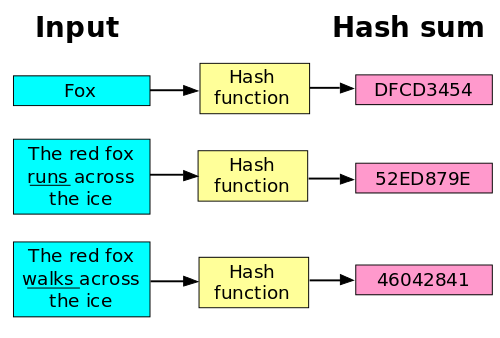
\includegraphics[scale=0.35]{hash_function}
	\caption{TODO citar wiki}
	\label{fig:hash}
\end{figure}

As funções de sentido único tem diversas utilidades na área de computação,
desde na busca de dados em uma estrutura de dados chamado de tabela hash, que
possibilita consultas de forma rápida, até na parte de banco de dados, que é
possível a detecção de registros duplicados ou até mesmo a não integridade de
determinado dado.

Na área de criptografia há ainda a utilização em assinaturas digitais, códigos
de autenticação de mensagens, e ainda outras formas de autenticação. Além do
mais é  muito utilizada em \textit{blockchains}, com sua finalidade em fornecer
prova de trabalho e outras propriedades como utilizar um endereço sem revelar
sua chave pública e consequentemente sua privacidade.\cite{hashBlockchain}

\section{Criptografia homomórfica}

A ideia de usar homomorfismo na criptografia surgiu em um trabalho científico
publicado com o objetivo de propor um criptossistema em um cenário de aumento
da utilização de terminais remotos. Neste caso, não seria ideal ter acesso a
todo o banco de dados cifrados e então decifrá-los para trabalhar os dados.
Neste contexto, surge o conceito de se operar com dados cifrados e obter-se o
mesmo resultado caso se estivesse operando em texto plano.\cite{homomorphic}

Criptografia homomórfica inclui diversos tipos de esquemas de criptografia que
podem ser executados em diferentes classes de dados cifrados. Os tipos mais
comuns de homomorfismo em criptografia são parcialmente homomórfico,
relativamente homomórfico e completamente homomórfico.\cite{survey-homo}

O nome criptografia homomórfica é derivado do conceito de homomorfismo em
álgebra abstrata. Um homomorfismo é uma aplicação que preserva a estrutura
entre duas estruturas algébricas X e Z.

\begin{equation}
f : X \longrightarrow Y
\end{equation}

Seja $\alpha$ uma função de ciframento e $\beta$ uma função de desencriptação
correspondente. Sejam $x1$, $x2$ dados em texto plano. A tupla ($\alpha$,
$\beta$) é uma cifra homomórfica com o operador $\star$ se a propriedade for
satisfeita:

\begin{equation}
\beta (\alpha(x1)) \star (\alpha(x2)) = x1 \star x2
\end{equation}

As operações principais de um esquema homomórfico de criptografia são:
\textit{KeyGen}, \textit{Encryption}, \textit{Decryption}, \textit{Eval}.
\textit{KeyGen} é a operação para criar uma chave pública e outra privada em uma
versão de criptografia assimétrica e a criação de uma chave única em modelo
simétrico. \textit{KeyGen}, \textit{Encryption}, \textit{Decryption} não são
diferentes de suas funções em seus modelos tradicionais.  Entretanto,
\textit{Eval} é uma operação específica de sistemas homomórficos, que tem como
entrada e saída textos cifrados, adicionalmente, o dado cifrado resultante não
deve aumentar de tamanho, caso contrário, haveria um limite de operações
possíveis.\cite{survey-homo}

\begin{figure}[h]
	\centering
	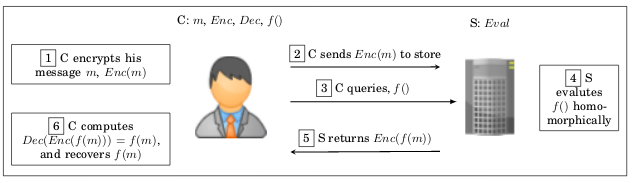
\includegraphics[scale=0.4]{crypto-homo}
	\caption{Imagem tirada do paper ACAR et al., 2018.}
	\label{fig:crypto-homo}
\end{figure}


\section{Blockchain}

Da sua tradução literal, blockchain significa cadeia de blocos. De  maneira
simplista, pode ser definido como um bloco ligado com o anterior, gerando assim
uma cadeia. Estes blocos carregam as informações que são importantes para a
rede. No caso de uma criptomoeda como \textit{Bitcoin}, cada bloco teria dados
sobre as transações realizadas naquele dado instante, ou seja, uma definição do
estado atual do sistema.

A concepção da blockchain foi feita para ser um encadeamento de registros
imutáveis, distribuídos e públicos. Os registros são imutáveis devido ao tipo de
encadeamento que é feito com os blocos, em que o ponteiro para o bloco anterior
é projetado para garantir a imutabilidade dos dados. Como é um protocolo
distribuído, todas as informações não estão armazenadas em um servidor central e
não há um nodo mestre que coordene a rede. Justamente o oposto disso, a
blockchain está replicada em todos os nodos participantes da rede, que podem
estar espalhados pelo mundo inteiro. Além de ser um esquema distribuído, o
referido também é público, pois não há como censurar uma parte de participar da
rede, basta o interessado ter acesso a internet que ele poderá realizar a sua
cópia da base de dados.\cite{blockchain}

\subsection{Cadeia de blocos}
A estrutura de um bloco pode variar de acordo com a necessidade e propósitos da
cadeia de blocos, vamos tomar como exemplo a cadeia do \textit{Bitcoin}, visto
que foi a primeira a ser criada e até hoje é mais importante e mais utilizada.
A estrutura de um bloco é basicamente a seguinte:

\begin{itemize}
	\item Constante de valor 0xD9B4BEF9.
	\item Tamanho do bloco em \textit{bytes}.
	\item Cabeçalho do bloco, que consiste em 6 itens.
	\item Quantidade de transações no bloco.
	\item Transações em si.
\end{itemize}

Vale notar que as transações detêm uma estrutura de dados que permite a criação
de \textit{scripts}, além de permitir a inserção de dados arbitrários. \\

Já a estrutura do cabeçalho do bloco é composta por:
\begin{itemize}
	\item Versão do bloco.
	\item \textit{Hash} do bloco anterior.
	\item \textit{Hash} do bloco atual, baseado em todas as transações do bloco.
	\item \textit{Timestamp} em que o bloco foi criado.
	\item \textit{Nonce}, número aleatório que é utilizado na mineração dos blocos.
	\item \textit{Bits}, objetivo atual da mineração em formato compactado.
\end{itemize}

Esta estrutura de dados permite que qualquer participante da rede possa validar
o bloco de maneira rápida. Existe o desafio matemático para a criação de blocos,
isto é, para criar um novo bloco, ele deve calcular um \textit{Hash} com uma
pseudo colisão de acordo com a variável \textit{Bits} do cabeçalho. Resolver
esse desafio matemático é chamado de mineração, e a cada bloco que passa se
torna mais difícil, entretanto, uma vez que sua solução é conhecida, é
extremamente fácil de validar sua corretude. Há diversas soluções possíveis para
determinado bloco, porém é necessário que apenas uma seja
encontrada.\cite{Antonopoulos}

Como a mineração de blocos se torna cada vez mais difícil, a probabilidade de
algum atacante conseguir reescrever um bloco anterior é mínima, visto que ele
teria que concluir o desafio matemático para o bloco que deseja modificar e
ainda todos os sucessores dele.

\begin{figure}[h]
	\centering
	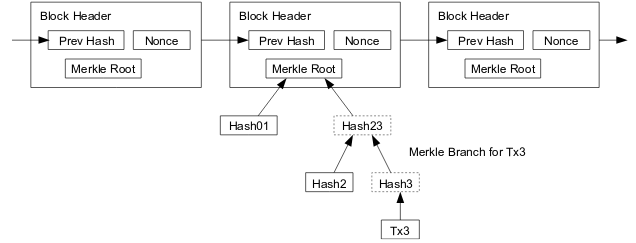
\includegraphics[scale=0.4]{blockchain}
	\caption{Imagem tirada do whitepaper do Bitcoin.}
	\label{fig:blockchain}
\end{figure}

\section{Contratos inteligentes} A ideia de contrato sempre esteve presente
durante todo o curso da humanidade, com a evolução da sociedade foi se criando
novos conceitos para se formalizar uma relação. O contrato é o pilar das
relações econômicas modernas. Entretanto esse mecanismo tem um custo elevado,
durante o processo de criação e utilização de contratos, normalmente baseados em
lei comum, que muitas vezes torna-se inviável para determinados casos.

Idealizado no ano de 1997 por Nick Szabo, os contratos inteligentes foram
pensados como uma substituição natural dos contratos realizados no cotidiano.
Em analogia, a ideia é utilizar de software e hardware para a tomada de
decisões, como em uma máquina automática de vendas de refrigerante. Os
contratos inteligentes vão além da máquina de vendas, uma proposta de
utilização de contratos em todos os tipos de propriedade e controlado do meio
digital. Eles possibilitam a verificação desse contrato de maneira dinâmica e
proativa.\cite{szabo-smart}

Já no surgimento da blockchain descrito no protocolo do Bitcoin, havia espaço
para criação de \textit{scripts} nas transações. Entretanto, estes
\textit{scripts} foram concebidos para serem simples, com a ideia de não
sobrecarregar a rede com a execução de códigos complexos. Um exemplo de
\textit{script} trivial seria o congelamento de fundos até certa data futura.
Como não são  permitido \textit{loops} em sua estrutura, isto impacta na não
Turing completude da linguagem de \textit{script}.\cite{nakamoto2012bitcoin}

Almejando-se ter \textit{scripts} mais potentes, foi criado o conceito de
contratos inteligentes, que são Turing-completos e ainda podem guardar o estado
atual do sistema.  Assim, possibilita a criação de aplicações extremamente mais
complexas.\cite{ethereum}

A \textit{blockchain Ethereum} foi criada juntamente com sua \textit{Virtual
Machine}, a EVM\sigla{EVM}{\emph{Ethereum Virtual Machine}} como é chamada, que
utiliza de um vasto conjunto de instruções para executar tanto tarefas
específicas quanto gerais. Para armazenar os conjuntos de instruções de forma
eficiente, a EVM os codifica em \textit{bytecodes}.\cite{wood2014yellow}

Consequentemente com a criação do conjunto de instruções, houve a criação da uma
linguagem de programação de alto nível que é compilada para esses
\textit{bytecodes} específicos.  \textit{Solidity} foi criada para ser uma
linguagem simples de ser entendida e reproduzida para quem já têm os
conhecimentos de programação de outras linguagens padrões de alto nível.
\cite{solidity}

\begin{figure}[h]
	\centering
	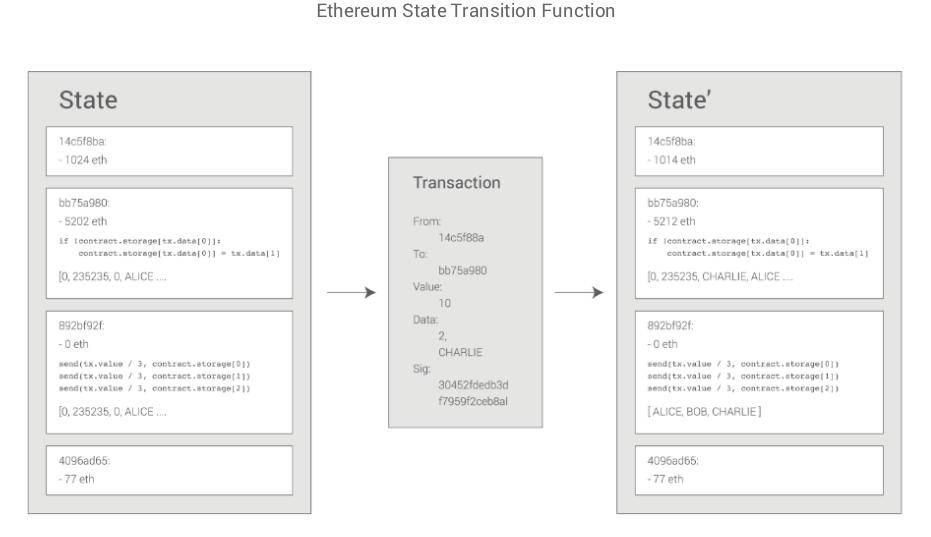
\includegraphics[scale=0.3]{ethereum}
	\caption{Imagem tirada do whitepaper Ethereum}
	\label{fig:ethereum}
\end{figure}

Desta forma, é possível criar aplicações que rodam de forma descentralizada e
que podem ter seu estado atual verificado por qualquer participante do sistema
em qualquer momento além de garantir as propriedades da blockchain.

\chapter{Helios}

\section{Introdução}

Neste capítulo será apresentado o software Helios voting, em que este trabalho
se baseia para criar um módulo \textit{blockchain} para realizar a prova de
existência das informações importantes para a verificação e auditoria de uma
eleição neste software.

\section{Sobre}

Helios voting é um software de código aberto desenvolvido por Ben Adida. Foi
desenvolvido com o intuito de ser o primeiro aplicativo baseado na
\textit{Web}, de auditoria aberta ao público. De maneira que qualquer um
poderia rodar sua própria eleição, e quem estiver disposto a observar o
processo e auditar o processo inteiro conseguiria também. É concebido para ser
usado em clubes locais, eleições para reitor de universidade e comunidades
online. De maneira votos secretos são necessários e a coerção não é um grande
problema.\cite{benAdida}

O código do front-end foi escrito em \textit{JavaScript} e \textit{HTML}, e a
parte do servidor foi desenvolvida em \textit{Python} com o framework para
aplicações web \textit{Django}. 

Algumas características do esquema proposto:

\begin{itemize}

	\item Eleições com baixa coerção: Votações online e por carta sempre
		tiveram um problema de coerção, visto que, nessa abordagem é possível
		que na hora do voto, há outra pessoa forçando por meio de ameaças ou
		força física a maneira que a pessoa vote. Alguns sistemas possibilitem
		que o voto seja feito mais de uma vez para mitigar esse problema,
		assim, a coerção deveria ocorrer durante todo o período da eleição para
		ter sucesso. A abordagem do Helios é que o último voto é sempre o
		válido para a eleição, de forma que se a eleição for feita em período
		de intervalo de dias, é difícil ter uma coerção de uma maioria
		significativa para o resultado. Dessa forma, essa abordagem visa apenas
		eleições onde o que está jogo não é algo tão crítico, como uma votação
		para o presidente de um país.
	\item Não confie em ninguém para integridade, confie no Helios para
		privacidade: Criptossistemas de voto eletrônico possuem duas
		propriedades que devem proteger, tanto a privacidade do voto, quanto a
		integridade. Num modelo de ataque onde todas as partes do sistema é
		corrompido e atacado, existe o entendimento que não há como proteger as
		duas coisas ao mesmo tempo. A abordagem do Helios acredita que é mais
		importante que a integridade seja garantida. Dessa forma, há a
		necessidade que um conjunto minimo de administradores/apuradores sejam
		honestos para que a privacidade não seja comprometida, entretanto mesmo
		que todos apuradores sejam maliciosos, isso não afeta a parte de
		auditoria do sistema. Portanto há a necessidade de se confiar na infraestrutura do Helios
		para que a privacidade seja garantida.

\end{itemize}

\section{Processo de voto}

O primeiro passo é criar uma eleição, para isso, o usuário deve ter uma conta
no Helios, que requer um email, nome e senha. O usuário pode então criar uma
eleição com um determinado nome e define o período de votação. Desta forma o
usuário que criou a eleição se torna um administrador da mesma. Uma vez que a
eleição é criada, o Helios já provêm todas as chaves criptográficas necessárias
para o esquema. O administrador prepara então a cabine de votação com as
perguntas e respostas, além de carregar todos os eleitores aptos para a
eleição, essas informações podem ser editadas até o momento que a votação
comece. O administrador deve congelar a eleição quando a mesma está pronta para
receber os votos. Uma vez congelada, nada pode ser alterado sobre a cabine,
votantes ou tempo da eleição.


Um outro usuário que foi adicionado como um eleitor pelo administrador,
receberá em seu email o seu usuário da eleição, uma senha gerada aleatória que
é específica para esta votação e um link para a cabine de votação online, além
de um resumo criptográfico dos parâmetros da eleição para fins de auditoria.
Assim que iniciar o processo de votação na cabine pelo link recebido, o mesmo
faz a escolha de seus votos e por fim realiza uma revisão de suas decisões. Uma
vez revisado a cédula de votação, ela é selada e então cifrada para enviar para
o servidor.

Assim que o voto é cifrado, há a possibilidade do eleitor auditar o texto
cifrado para verificar se realmente o seu voto foi computado corretamente.
Entretanto uma vez que o voto cifrado é aberto, é necessário que seja cifrado
novamente. Nesta hora é realizado o processo de autenticação do eleitor, caso a
autenticação for um sucesso, a cédula é adicionada na eleição pelo servidor.
Todos os votos são publicados em um boletim, que contêm o identificador do
votante junto com seu voto cifrado.

Quando a eleição acabar, o servidor embaralha todas as cédulas, cifra todos os
votos e coloca de modo público para as partes interessadas em auditar a
votação. A auditoria permite verificar que o embaralhamento dos votos foi feito
de maneira correta. Depois de um certo período de tempo, o Helios decifra as
cédulas de votação e registra os votos. Qualquer pessoa pode baixar os dados
gerados pela eleição para verificar que o embaralhamento, decifragem e contagem
estão corretos.

Vale ressaltar aqui que o voto individual nunca é decifrado de maneira
individual, uma vez que apenas os votos cifrados são encaminhados para o servidor,
então é utilizado de criptografia homomórfica para combinar todos os votos
cifrados em uma coisa só, a contagem,  e apenas a contagem é decifrada, não
revelando nenhuma informação adicional, a não ser pelo resultado.

\section{Informações relevantes para auditoria}

\lstset{
    string=[s]{"}{"},
    stringstyle=\color{blue},
    comment=[l]{:},
    commentstyle=\color{black},
}

O esquema proposto pelo Helios já provêm diversas garantias para que sua
auditoria seja realizada de forma transparente e aberta ao público.
Disponibiliza diversos \textit{endpoints} que fornecerem informações relevantes
para a verificação da eleição. Como a lista dos eleitores aptos, de forma que
essa lista pode ser por meios de pseudônimos para evitar a divulgação de
informações, mas caso a lista seja pública, não há a necessidade de se utilizar
pseudônimos. Todas as informações são disponibilizadas em formato JSON.

Exemplo de lista de eleitores

\begin{lstlisting}[numbers=none]
[
   {
      "id":"vinicius.macelai@gmail.com",
      "name":"Vinicius Macelai",
      "type":"email",
      "uuid":"60435862-65e3-11de-8c90-001b63948875"
   },
   {
      "id":"ben@adida.net",
      "name":"Ben2 Adida",
      "type":"email",
      "uuid":"4e8674e2-65e3-11de-8c90-001b63948875"
   }
   ...
]
\end{lstlisting}

Há também um \textit{endpoint} que disponibiliza todas as questões da eleição, essa também é uma informação relevante para auditoria, visto que, uma vez publicado essas informações, teoricamente não deveria ser possível de se alterar qualquer dado de uma das questões. Sendo necessário guardar esse histórico para comparar com o que realmente aconteceu.

Exemplo da estrutura das questões

\begin{lstlisting}[numbers=none]

[
   {
      "answer_urls":[
         "",
         ""
      ],
      "answers":[
         "Sim",
         "Nao"
      ],
      "choice_type":"approval",
      "max":1,
      "min":0,
      "question":"Pergunta 1",
      "result_type":"absoluta",
      "short_name":"Pergunta 1",
      "tally_type":"homomorphic"
   },
   {
      "answer_urls":[
         "",
         ""
      ],
      "answers":[
         "Nao",
         "Sim"
      ],
      "choice_type":"approval",
      "max":1,
      "min":1,
      "question":"Segunda pergunta",
      "result_type":"absoluta",
      "short_name":"Segunda pergunta",
      "tally_type":"homomorphic"
   }
   ...
]

\end{lstlisting}

Já para os votos, há um outro \textit{endpoint} que revela algumas informações
sobre os votos, não há como acessar o voto de maneira clara, nem mesmo cifrado.
Apenas é possível verificar a hora que foi votado, o hash do voto e do eleitor,
e a identificação do eleitor. Isto é importante para verificar que um
determinado foi computado e não excluído, além de ser possível, relacionar o
identificador do eleitor na tabela de votantes, para saber que nenhuma pessoa
que não era apta a votar, votou.

Exemplo da estrutura de um voto.
\begin{lstlisting}[numbers=none]

[
 {
    "cast_at": "2019-10-10 10:44:27.622007",
    "vote_hash": "ii3clNdJarrMZ+du5t9xRe5m3+agnrm67YSsdIwPRHs",
    "voter_hash": "1HY5y0fXMqxapWNqCf82K2BpVrAWPKmtS9hN5YqL7jc",
    "voter_uuid": "c0157d63-b7a9-49e9-8021-9d35d3c83ea9"
  }
  ...
]

\end{lstlisting}

Para os dados gerais da eleição, há um \textit{endpoint} que disponibiliza
várias informações sobre a votação. Como o nome da votação, sua descrição, a
hora que a eleição foi congelada para dar início aos votos, a sua chave pública
que é utilizada na hora da verificação dos votos, hash dos eleitores, hora de
início e fim da votação. São várias informações que são úteis em uma auditoria,
pois é possível verificar se alguma coisa não aconteceu conforme o que o
público geral esperasse.


\begin{lstlisting}[numbers=none]

{
   "cast_url":"https://e-democracia.ufsc.br/helios/elections/e64c77be-e6dd-11e9-9ed0-0050568db9bc/cast",
   "description":"",
   "frozen_at":"2019-10-10 13:56:23.825227+00:00",
   "name":"teste",
   "openreg":true,
   "public_key":{
	  "g":"1488749222496318763428242153718604080130
	  400801774349230448173738257193393756872447384
	  710602991504015078403188220609028693866146445
	  889649421527398954788920114485735261105857223
	  657873431950512804260237286457042655085520144
	  811174657987181124911478167430906269344244236
	  869744997064823262188000170953514304791366143
	  288328715000342980239222936158360868664324334
	  972779197624724794861893042386618041055845827
	  260662711127004009120307358023890530399447220
	  293078320747239457849850776470319128824954765
	  989999713116613025970060443389123229818234840
	  317594745028443341126596678913102457362954604
	  8637848902243503970966798589660808533",
	  "p":"1632863208493301000238405503380545732960
	  161477118595538973916730908621480040646579903
	  858363495375294167564556218249812075026498049
	  238137557936767564877129380031037096474576701
	  424363851844255382397348299526730404432677704
	  766295748026939132278937838461942859644644698
	  469430618764476746246096562258008756433921263
	  177581789595840901667639897567126617963789855
	  768731707617721884323315069515788106125705301
	  913307854592898356222139631316962247550981844
	  266104701843626480690102396623671836720471075
	  593589901375030610773800236413791742659573740
	  387111418775080434656473125060919684663818390
	  3982387884578266136503697493474682071",
	  "q":"6132956624834290129254387276997895087063
	  3559608669337131139375508370458778917",
	  "y":"6674849462819707761425540060443321142147
	  065374239459835165544825432222893216813 43161
	  701912833679191861159511407066056382418705054
	  8693746028485084245830920486320377 0459478003
	  535479349067299809007231395222615550077332803
	  980377694907673841794062958485957445752678169
	  178233222755221822716717204325716622981245085
	  764017396596177317480111639095637201353649046
	  648287394475477034301481505230258754780469801
	  912243347674672857224825271821914019222712742
	  428353419223563690785390840589005731613775466
	  095536392298783449088276259415062502416297715
	  498188681306950146845971239763841785489152032
	  921279090551533346193693176660748711231231206"
	  },
   "short_name":"Teste_15",
   "use_voter_aliases":true,
   "uuid":"e64c77be-e6dd-11e9-9ed0-0050568db9bc",
   "voters_hash":"4496c913e4202e7bd165a3c6457bbef71081c07b",
   "voting_ends_at":"1570818542",
   "voting_starts_at":"1570811298"
}

\end{lstlisting}

Assim, o conjunto dessas informações, fornece uma transparência maior para o
processo de votação, de forma que uma auditoria externa poderia verificar se
houve alguma tentativa de manipulação da eleição. 

O problema atual dessa abordagem usando exclusivamente o Helios, é que se um
atacante consegue ter acesso ao servidor, consequentemente ele teria acesso ao
banco de dados da aplicação, com isto, o atacante poderia modificar qualquer
informação contida no mesmo. Por exemplo, a votação estava marcada para começar
em determinada hora, como mostrado anteriormente, o Helios necessita que um
administrador congele a eleição, de forma que nenhuma informação possa ser
modificada, o atacante então altera o horário de congelamento para uma data
futura, enquanto isso, ele pode realizar alterações nas configurações da
votação, como a exclusão ou adição de eleitores, de modo malicioso.


\chapter{Desenvolvimento}

Este capítulo será abordado a criação do esquema e desenvolvimento do projeto
proposto.

\section{Modificação do software Helios} 

Como mostrado no capítulo anterior, o Helios fornece diversas informações
relevantes para a auditoria de um processo de votação. Para acessar essas
informações, foram criados \textit{endpoits} para fornecer as informações, de
forma que, apenas as relevantes são buscadas, evitando redundâncias e
informações desnecessárias. Foi decidido de não alterar os \textit{endpoits}
originais para não causar uma pertubação no sistema. Para os votos, não foi
necessário nenhuma mudança no que já havia. Os criados foram:

\begin{itemize}
	\item GET `elections/<election\_uuid>/blockchain' retorna 
		informações públicas da eleição
	\item GET `elections/<election\_uuid>/blockchain/voters' retorna 
		informações públicas dos eleitores
	\item GET `elections/<election\_uuid>/blockchain/result' retorna
		informações sobre o resultado
\end{itemize}

Nas configurações do projeto, foi adicionado uma variável de ambiente contendo
o \textit{keystore}, que é um arquivo em formato JSON, com os dados de uma
carteira \textit{Ethereum}, contendo a chave privada, a cifra usada para
guardar a chave privada e os demais atributos.

\begin{lstlisting}[language=Python, numbers=none]
KEYSTORE = "/home/Helios/keystore.json"
KEYSTORE_PASSWORD = "TXv?m!U;9Q#%KMa"
\end{lstlisting}

Esse \textit{keystore} será usado para criar e assinar as transações e popular
os contratos com os dados da votação. Vale notar que a carteira já deve contar
com fundos necessários para arcar com o funcionamento dos contratos.

\section{Contratos inteligentes}

\subsection{Eleitores}

O contrato dos eleitores serve para basicamente saber qual é a lista os
eleitores, e o contrato pode variar de acordo com a votação.  Por exemplo,
existem eleições onde a privacidade dos dados dos eleitores deve ser
respeitada, de forma que seu nome e email não devem divulgados, para isso,
bastaria uma pequena mudança no contrato a seguir, alterando o nome para um
pseudônimo e a retirada do email.

\begin{lstlisting}[language=Solidity]
contract Voters{
    
    struct Voter {
        string uuid;
        string name;
        string email;
    }
    
    Voter[] public voters;
    
    function addVoter(string memory _uuid, string memory _name, string memory _email) public {
        voters.push(Voter(_uuid, _name, _email));
    }
}
\end{lstlisting}

Uma vez populado os eleitores no Helios, bastaria popula-los no contrato
também. Como já visto anteriormente, a lista de eleitores não pode ser
modificado uma vez que a eleição é congelada, portanto, uma adição de um
eleitor não qualificado para a eleição, não estaria nos dados do contrato,
constando uma fraude.

\subsection{Votos}

O contrato dos votos contêm uma peculiaridade, dado que será o único contrato
que não será populado pelo servidor Helios, visto que este será populado ao
decorrer do processo, diferente dos demais, os quais serão populados
previamente.  Essa decisão foi tomado levando em conta os seguintes aspectos,
caso o servidor do Helios fosse invadido, um atacante poderia não publicar o
voto, ou até mesmo, mudar o hash do voto para causar alguma confusão. 

A premissa é que o eleitor é honesto, tanto o esquema proposto pelo Helios,
quanto o desse trabalho, não há como garantir que caso algum votante alegue que
o seu voto não foi computado, ou aquele voto associado a ele não foi ele que
emitiu, não há como garantir ou provar nenhuma informação.

\begin{lstlisting}[language=Solidity]
contract Votes {
    
    struct Vote {
        string vote_hash;
        string voters_hash;
        uint256 cast_at;
    }
    
    Vote[] public votes;
    
    function addVote(string memory _vote_hash, string memory _voters_hash, uint256 _cast) public {
        votes.push(Vote(_vote_hash, _voters_hash, _cast));
    }
    
}
\end{lstlisting}

Vale notar aqui que o voto cifrado não é publicado, apenas o seu hash. Essa
decisão foi tomada pelo fato que a criptografia utilizada nos dias de hoje,
como ElGamal pode não ser segura no futuro, como já temos exemplos de
primitivas criptográficas no passado. CITAR PAPER

Partindo da premissa que o eleitor é honesto, então, isso seria uma prova que o
seu voto existiu em dado momento, e que, se ele não estiver na hora da apuração
do resultado, algo de errado houve com os votos, invalidando a votação.

\subsection{Eleição}

O contrato eleição é o principal, ele vai ser instanciado uma vez por votação e
o mesmo contêm os outros contratos instanciados como variáveis do contrato.
Além do mais irá conter as informações gerais sobre a votação, como o seu
\textit{uuid}, que é seu identificador único, o nome da votação, a URL que será
usada para votar, a data de criação, horário que irá abrir e fechar para os
votos, além de conter todas as perguntas e respostas e a chave pública da
votação, que é utilizada na hora da contagem e auditoria do votos, em provas de
conhecimento zero.

\begin{lstlisting}[language=Solidity]
contract Election {
    
    string public uuid;
    string public name;
    string public cast_url;
    uint256 public created_at;
    uint256 public frozen_at;
    uint256 public voting_starts;
    uint256 public voting_ends;
    
    struct Public_Key {
        string p;
        string q;
        string g;
        string y;
    }
    
    Public_Key public public_key;
    
    struct Question {
        string question;
        string[] anwsers;
    }
    
    Question[] public questions;
    
    Voters public voters_contract;
    Votes public votes_contract;
    Result public result_contract;
    
    constructor(string memory _uuid, string memory _name, string memory _cast_url, uint256 _created_at, uint256 _voting_starts, uint256 _voting_ends, uint256 _voting_ends, string memory _p, string memory _q, string memory _g, string memory _y) public {
        uuid = _uuid;
        name = _name;
        cast_url = _cast_url;
        created_at = _created_at;
        voting_starts = _voting_starts;
        voting_ends = _voting_ends;
        public_key = Public_Key(_p, _q, _g, _y);
        voters_contract = new Voters();
        votes_contract = new Votes();
        result_contract = new Result();
    }
    
    function addQuestion(string memory _question, string[] memory _anwsers) public {
        questions.push(Question(_question, _anwsers));
    }
    
}


\end{lstlisting}

Assim que configurado toda a votação, esse contrato seria populado com todos os dados da eleição


\subsection{Resultado}

O contrato do resultado é para divulgar o resultado individual de cada
pergunta, além do horário que foi divulgado, e o mais importante é o hash dos
eleitores, pois como o contrato dos eleitores foi populado previamente, é
possível calcular novamente, para saber que apenas os votantes que tinham
direito de votar, votaram.

\begin{lstlisting}[language=Solidity]
contract Result {
    
    struct Question {
        string question;
        int result;
    }
    
    Question[] public questions;
    string public voters_hash;
    uint256 public relesed_at;
    
    function addQuestion(string memory _question, int _result) public {
        questions.push(Question(_question, _result));
    }
    
    function setVotersHash(string memory _voters_hash) public {
        voters_hash = _voters_hash;
    }
    
    function setReleaseAt(uint256 _relesed_at) public {
        relesed_at = _relesed_at;
    }
}
\end{lstlisting}

\section{Fluxo de uma eleição}

Agora será mostrado, como seria o novo fluxo de eleição

No painel de administração de uma eleição, que só pode ser acessada por um usuário com privilégios, foi adicionado um botão para publicar os dados da eleição na blockchain.

\begin{figure}[H]
	\centering
	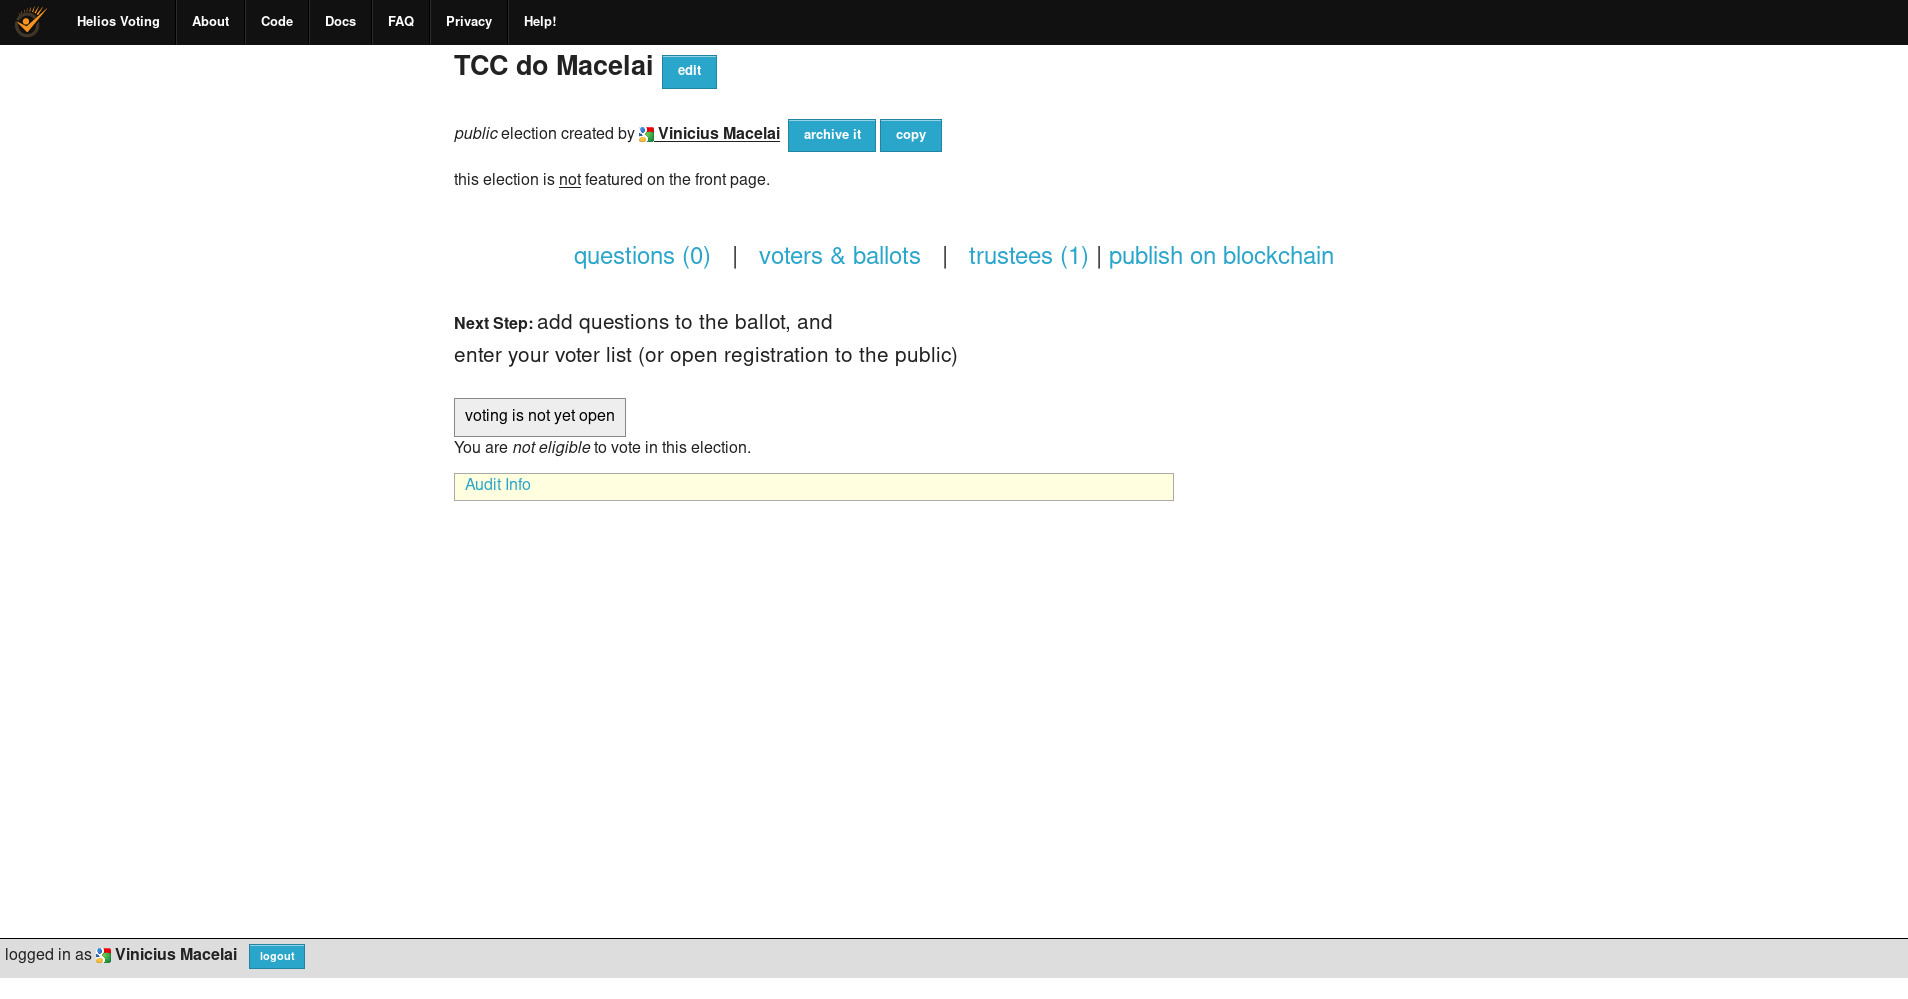
\includegraphics[width=\linewidth]{helios-1}
	\caption{Painel administrativo de uma eleição}
	\label{fig:helios-1}
\end{figure}

\begin{figure}[H]
	\centering
	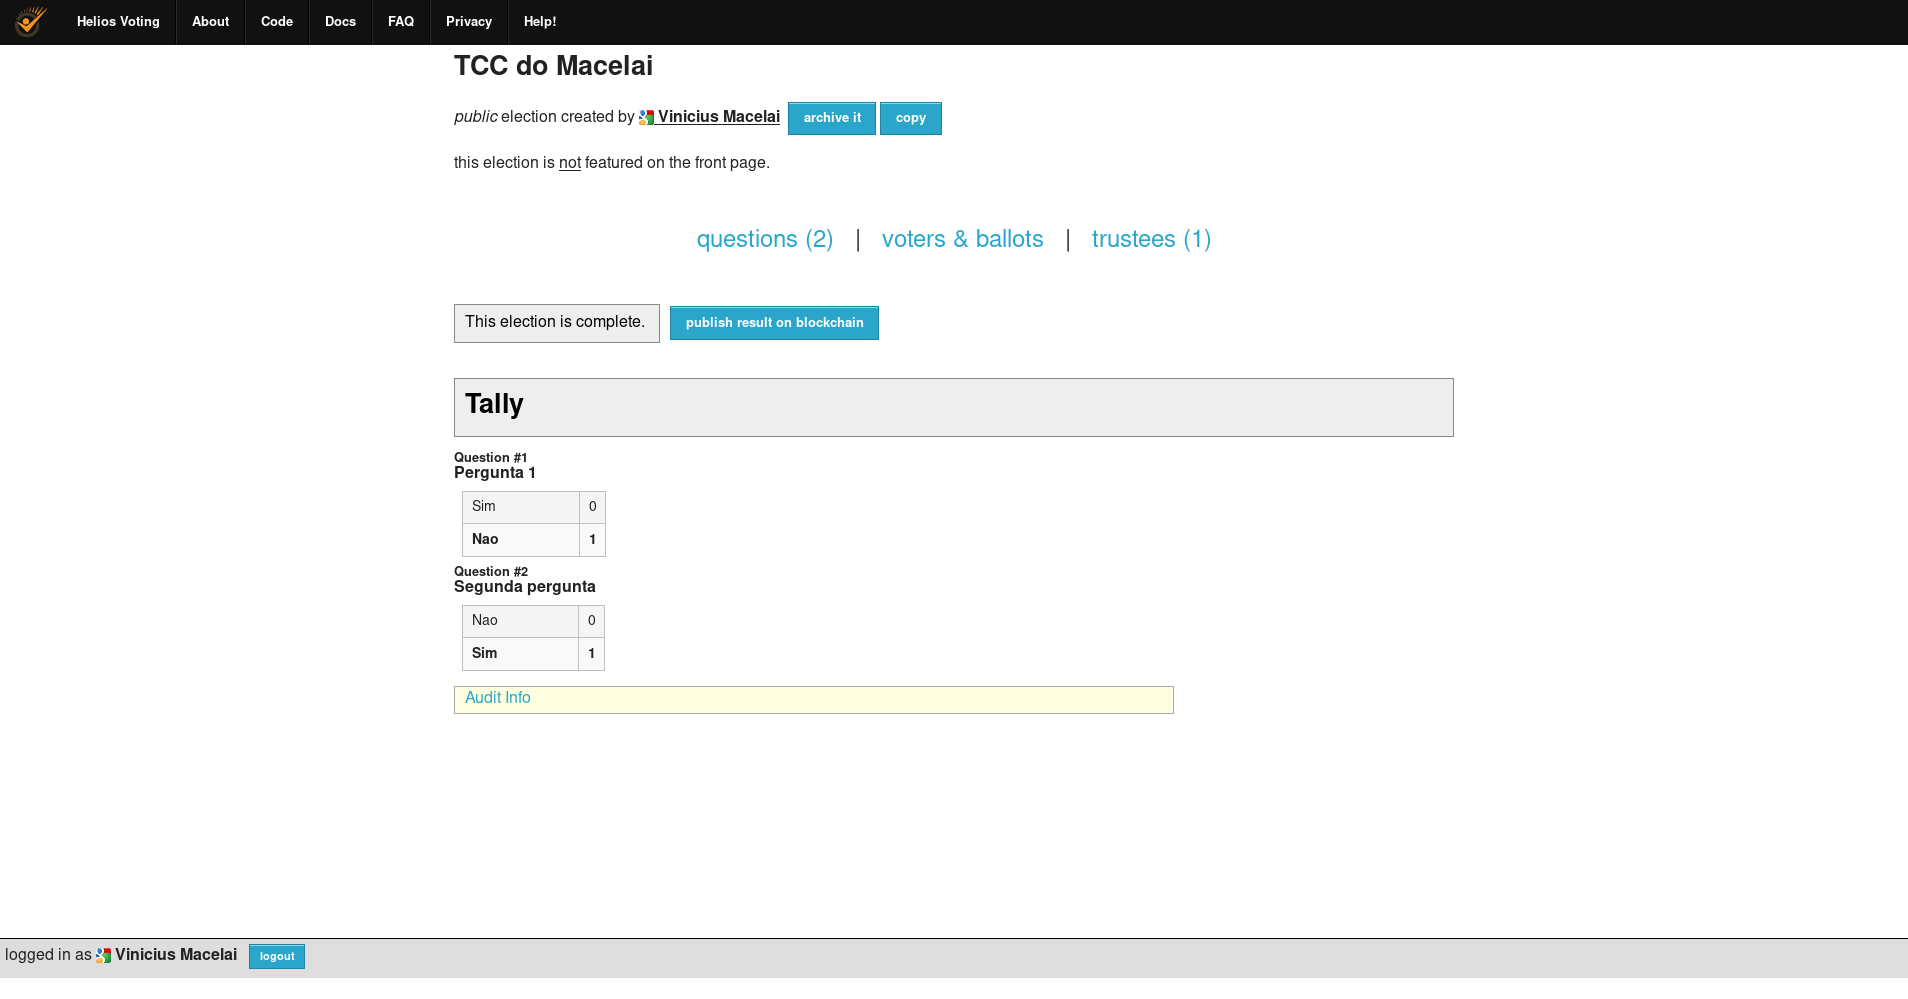
\includegraphics[width=\linewidth]{helios-2}
	\caption{Painel administrativo de resultado}
	\label{fig:helios-2}
\end{figure}


\section{Custo financeiro}

Nesta seção, estima-se os custos de transação cobrados para rodar na rede
principal da \textit{Ethereum}, de forma para rodar este protótipo.
Primeiramente, é estimado o custo individual de cada contrato, já que cada um
tem suas peculiaridades. Então é estimado e analisado em uma eleição hipotética
com mil eleitores.

Os construtores são as chamadas mais custosas, uma vez que são responsáveis por
instanciar memória não volátil na rede \textit{Ethereum}, que são as instruções
mais caras. Logo, o construtor do contrato "eleição" será o mais caro, pois ele
contêm todos os outros contratos em seus atributos.

Considerando o preço do \textit{Gas} utilizado em 25 \textit{gwei}, e o preço de um
\textit{Ether} em 169 dólares em média. Dados obtidos em 25/09/2019.

\begin{table}[htb]
\centering
\begin{tabular}{||c|c|c||}
\hline
	\textbf{Método}        & \textbf{Gas}    & \textbf{Dólar}  \\  [0.2ex] \hline \hline
constructor   & 571316 & \$2.41 \\
addQuestion   & 84624  & \$0.35 \\ 
setVotersHash & 87482  & \$0.36 \\ 
setReleasedAt & 42164  & \$0.17 \\ \hline
\end{tabular}
\caption{Custos do contrato resultado}
\label{tab:my-table}
\end{table}

\begin{table}[htb]
\centering
\begin{tabular}{||c|c|c||}
		\hline
		\textbf{Método} & \textbf{Gas} & \textbf{Dólar}  \\ [0.2ex] \hline \hline
		constructor & 389806 & \$1.64 \\ 
		addVote     & 128449 & \$0.54 \\ \hline
	\end{tabular}
	\caption{Custos do contrato votos}
	\label{tab:my-table}
\end{table}

\begin{table}[htb]
	\centering
	\begin{tabular}{||c|c|c||}
		\hline
		\textbf{Método}  & \textbf{Gas} & \textbf{Dólar}  \\ [0.2ex] \hline \hline
		constructor & 508588 & \$2.14 \\ 
		addVoter    & 151882 & \$0.64 \\ \hline
	\end{tabular}
	\caption{Custos do contrato votantes}
	\label{tab:my-table}
\end{table}

\begin{table}[htb]
	\centering
	\begin{tabular}{||c|c|c||}
		\hline
		\textbf{Método} & \textbf{Gas}  & \textbf{Dólar}   \\ [0.2ex] \hline \hline
		constructor & 2684091 & \$11.34 \\ 
		addQuestion & 129270  & \$0.54  \\ \hline
	\end{tabular}
	\caption{Custos do contrato eleição}
	\label{tab:my-table}
\end{table}

Agora, será estimado uma votação hipotética, composta por mil eleitores, três
questão e levando em consideração que a 10\% dos eleitores tenham votado duas
vezes, visto que é permitido votar mais de uma vez e é considerado apenas o
último. As chamadas para os contratos seriam a seguinte:

\begin{enumerate}
	\item 1x construtor do contrato eleição.
	\item 3x addQuestion do contrato eleição.
	\item 1000x addVoter do contrato eleitores.
	\item 1100x addVote do contrato votos.
	\item 3x addQuestion do contrato resultado.
	\item 1x setVotersHash do contrato resultado.
	\item 1x setReleasedAt do contrato resultado.
\end{enumerate}

Considerando os valores calculados nas tabelas anteriores temos um total de
\textbf{1248.54 Dólares} para rodar todo processo, até mesmo a divulgação do
resultado.

Fica claro que o maior custo está associado a adicionar os dados dos eleitores
e no momento de publicar a estrutra do voto. Dado que o custo para publicar os
outros dados, ficam marginais de acordo com a quantidade. Como é mostrado no
gráfico a seguir.

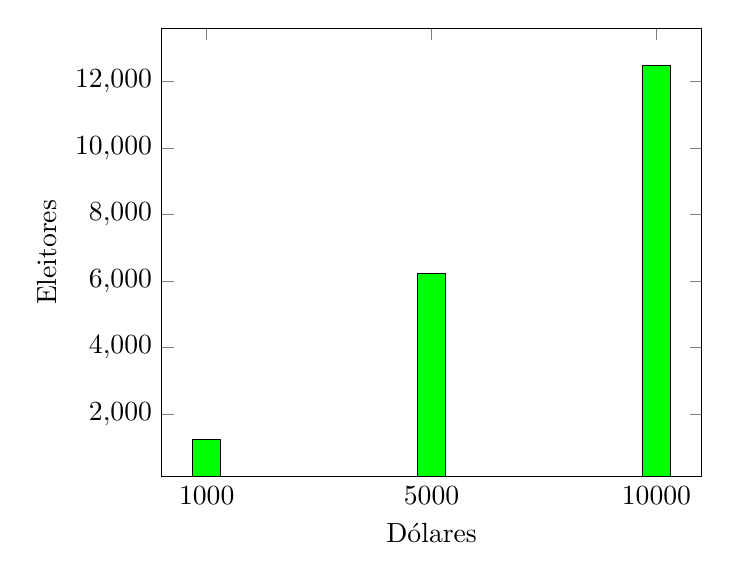
\begin{tikzpicture}{}
	\begin{axis}[
		symbolic x coords={1000, 5000, 10000},
		xtick=data,
		ylabel={Eleitores},
		xlabel={Dólares},
		yticklabel style={
        scaled y ticks = false, 
        scaled x ticks = false, 
        y tick label style={/pgf/number format/.cd, fixed, fixed zerofill,
                            int detect,1000 sep={\;},precision=3},
        x tick label style={/pgf/number format/.cd, fixed, fixed zerofill,
                            int detect, 1000 sep={},precision=3}
			},
	  ]
		\addplot[ybar,fill=green] coordinates {
			(1000,   1248)
			(5000,  6240)
			(10000, 12480)
		};
	\end{axis}
\end{tikzpicture}

\chapter{Conclusão}
Neste trabalho, foi desenvolvido um esquema e uma implementação de um módulo
para garantir maior auditabilidade e transparência para o sistema de eleição
online Helios, com a utilização da \textit{blockchain} para garantir a
imutabilidade dos dados inseridos. 

Uma conclusão muito importante feito a partir da análise de custos do modelo
proposto. Foi que há um custo relativamente elevado para rodar o modelo. Desta
forma, dependendo do caso de uso da eleição, não há a necessidade de se ter
tanta segurança no processo, de forma que o custo se torne incompatível com as
necessidades.  Entretanto, para votações onde já há um custo elevado para a
realização da mesma, há a possibilidade de se alterar para utilização do Helios
junto com módulo desenvolvido para se ter maior segurança para o processo de
votação, sendo um caso de uso legítimo.

A pergunta da pesquisa pode ser respondida a partir dos dados obtidos do modelo
construído, conjuntamente com as hipóteses propostas, de forma que foi criado
um módulo utilizando \textit{blockchain} para garantir auditabilidade. Foi feito
estudo do custo para o volume de dados. Além de discutido se esse modelo é
economicamente viável.

\section{Trabalhos futuros} 

A construção dos contratos inteligentes mostrou que há um custo muito alto
associado aos contratos, de forma que a otimização dos mesmos possa reduzir o
custo. Podendo ser otimizado de acordo com a necessidade do processo de
votação, como excluir certas informações dos contratos. Outra coisa a ser
levada em conta é a maturidade das linguagens de programação para os contratos,
de forma que, com a maturidade dessas linguagens, poderá ser feito de maneira
mais otimizada.

Outra possibilidade para a avaliação de redução de custos seria a utilização de
outras \textit{blockchains}, visto que, cada uma detêm de características
próprias, podendo reduzir o custo e possivelmente realizar uma abordagem mais
completa do processo de auditoria.

Um aspecto não abordado nesse trabalho, é parte da verificação matemática dos
votos. Como mostrado anteriormente, o Helios fornece todas as informações para
uma auditoria externa, e nessa abordagem não lidamos com os votos cifrados.  Um
dos motivos é que a verificação é extremamente custosa computacionalmente e
exige diversas manipulações dos dados. Além do mais, a linguagem utilizada na
criação dos contratos inteligentes não tem maturidade suficiente para ser
possível realizar toda essa computação.

Uma abordagem mais completa ainda, seria a completa substituição do Helios por
contratos inteligentes, de maneira que o contrato seria responsável por todas
as partes do processo de votação, como a autenticação dos eleitores, além de
fazer a contagem dos votos e divulgação dos resultados. Seria um modelo
completamente descentralizado, trazendo diversas vantagens para o esquema,
porém, com a imaturidade da tecnologia \textit{blockchain} e de contratos
inteligentes, isso se torna extremamente difícil no momento.

\bibliographystyle{abnt-alf}
\bibliography{ref}

\apendice{}

\chapter{ARTIGO DO TCC}

\end{document}
